\documentclass[english,version-2020-11]{uzl-thesis}

\UzLThesisSetup{
  Masterarbeit,
  Logo-Dateiname        = {uzl-thesis-logo-itcs.pdf},
  Verfasst              = {am}{Institut für Theoretische Informatik},
  Titel auf Deutsch     = {Über elementare Eigenschaften einer mehrdimensionalen Verallgemeinerung des euklidischen Algorithmus},
  Titel auf Englisch    = {On Elementary Properties of a Multi-Dimensional Generalization of the Euclidean Algorithm},
  Autor                 = {Daniel Knaack},
  Betreuerin            = {Prof. Dr. Kim-Manuel Klein},
  Studiengang           = {Informatik},
  Datum                 = {18. Juni 2025},
  Abstract              = {TODO},
  Zusammenfassung       = {TODO},
  Numerische Bibliographie,
}

\UzLStyle{pagella contrast design}

\usepackage{standalone}
\usepackage{todonotes}
\usepackage{mathtools}

\usetikzlibrary{decorations.pathreplacing, calligraphy}

\newcommand\N{{\mathbb N}}
\newcommand\Z{{\mathbb Z}}
\newcommand\Q{{\mathbb Q}}
\DeclareMathOperator*{\argmin}{arg\,min}
\DeclareMathOperator*{\argmax}{arg\,max}
\DeclarePairedDelimiter\ceil{\lceil}{\rceil}
\DeclarePairedDelimiter\floor{\lfloor}{\rfloor}

\begin{document}

\chapter{Introduction}
\label{ch:intro}

In 1839, Charles Hermite wrote a letter to Jacobi~\cite{Hermite50} about the
representation of real numbers.
He asked, whether there exists a representation of the real numbers as a
sequence of integers, which is periodic if and only if the represented number
is a cubic irrational, i.e. the root of a cubic polynomial.
Although he posed the question nearly two centuries ago,
it remains unanswered to this day.

The standard way to represent numbers is through decimal notation.
A number is represented as a sequence of digits, which begins with the integer
part and is followed by a (potentially infinite) sequence of digits for the
fractional part.
If the decimal expansion of a number is finite, then the number is clearly rational.
Furthermore, if the decimal expansion is periodic, then the number is rational, too.
The same behavior occurs for continued fractions and quadratic irrationals.
Continued fractions are fractions of the form
\[
  a₀ + \cfrac{1}{a₁ + \cfrac{1}{a₂ + \cfrac{1}{⋱}}},
\]
where $a₀, a₁, a₂, …$ are integers.
Any real number has a continued fraction expansion,
which can be constructed using the Euclidean algorithm.
If that continued fraction is periodic, then the number must be a quadratic irrational.
More importantly, the converse is also true:
If a number is a quadratic irrational,
then its continued fraction must be eventually periodic.
Naturally, we can ask whether we can extend this and
find a periodic representation for cubic irrationals.
However, no such representation exists as of yet.

The interest in a generalization to cubic irrationals
comes from the effectiveness of continued fractions in related fields.
The primary example is Diophantine approximation, where the goal is to
approximate real numbers using rational numbers as closely as possible.
It turns out that the best rational approximations are exactly those provided
by continued fractions.
A generalization of continued fractions could serve a similar role in the field
of simultaneous Diophantine approximation, where the goal is to approximate
multiple real numbers at once with a single rational vector.

Hermite's original question only applies to cubic irrationals,
but it can be easily generalized to any algebraic number:
Does there exist a representation of the real numbers as a sequence of integers
that is periodic if and only if the represented number is a algebraic number of
degree $d$?
There are two parts to this question.
The first is the representation of real numbers as a sequence of integers.
Each finite subsequence of the representation should give us a rational number,
which approaches the represented number as the sequence grows larger.
The second part is about the periodicity of the integer sequence.
In the original question, the sequence should repeat after some point if and
only if the represented is a cubic irrational.
The general question asks whether a periodic sequence exists for any algebraic
number with a certain degree.

% ==============================================================================
\section{Background}
\label{sec:jacobi-perron}
% ==============================================================================

Since Hermite originally posed his question to Jacobi, it was he who first
attempted to answer it.
He developed an algorithm \cite{Jacobi68} inspired by the Euclidean algorithm,
which calculates the greatest common divisor of three numbers instead of two.
At each step,
the algorithm chooses the smallest number and uses it to divide the other two.
In the next triple, the other two numbers are replaced by their remainder.
This process is continued until the greatest common divisor is found.
Later, Oskar Perron generalized Jacobi's method to arbitrary dimensions \cite{Perron07},
resulting in what is now called the Jacobi–Perron Algorithm (JPA).
His algorithm is essentially a generalization of the Euclidean algorithm to $n$ numbers.
At each step, he still chooses the smallest element at each iteration.

Continued fractions are typically constructed using the Gauss transformation,
which is defined as
\begin{align*}
  T(x) = \frac{1}{x - \floor{x}}.
\end{align*}
This transformation is applied repeatedly until $T^m(x) = T^n(x)$ for $m ≠ n$,
in which case the continued fraction is periodic.
The Jacobi-Perron uses a similar transform,
which takes a vector $x = (x₁, …, x_d)$ as input and calculates
\begin{align*}
  T(x₁, …, x_d) =
  \left(
  \frac{x_2 - \floor{x_2}}{x_1 - \floor{x_1}},
  \frac{x_3 - \floor{x_3}}{x_1 - \floor{x_1}},
  …,
  \frac{x_d - \floor{x_d}}{x_1 - \floor{x_1}},
  \frac{1}{x_1 - \floor{x_1}}
  \right)
\end{align*}
Again, this transformation is applied repeatedly until $T^m(x) = T^n(x)$ for $m ≠ n$,
at which point it becomes periodic.
However, Perron has only shown one direction:
If the algorithm becomes periodic, then $x$ is an algebraic number with degree $d+1$.
In an attempt to find an algorithm, which solves both directions,
previous work often replaces this transformation with a different one,
which can be considered JPA-type algorithms.
For example, a different transformation could use the second smallest number.
They usually consider only one particular transformation and iterate this until a period has been found.
Despite numerous different transformations being proposed,
Hermite's question remains open.

% ==============================================================================
\section{Contributions of this Thesis}
\label{sec:contributions}
% ==============================================================================

% The other algorithms focus on a single path, whereby the only use their own
% transformation function to find a periodic representation.
This thesis extends previous work on multidimensional continued fractions (MCFs).
The JPA usually only considers the smallest number in each iteration,
however there are algorithms based on the JPA which choose a different number,
like choosing the largest number \cite{Podsypanin77} or choosing some number
based on a cost function \cite{Tamura09}.
In this thesis, I present a whole class of MCFs,
which encompass all JPA-type algorithms.
The main contributions regarding these MCFs are as follows:
\begin{enumerate}
  \item \textbf{Convergence}:
    I establish sufficient conditions under which the proposed class of MCFs
    algorithms converges.
    This generalizes known convergence results for the JPA to a wider family of
    transformations and solves the first part of Hermite's question.
  \item \textbf{Algebraicity from Periodicity}:
    I prove that if a multidimensional continued fraction expansion becomes
    eventually periodic, then the original input vector consists of algebraic
    numbers.
    This solves one direction for the second part of Hermite's question.
    It still leaves open the question whether algebraic numbers always lead to
    periodic MCFs.
\end{enumerate}

In addition to these theoretical results,
I have performed an experimental analysis on the MCFs.
The aim of this analysis was to see which strategies could be used
to construct periodic MCFs for algebraic numbers
and I provide a comparison of existing JPA-type algorithms,
which can be used for constructing MCFs of cubic and quartic irrationals.
One strategy shows particular promise in the construction,
since it has provided a periodic MCF for any cubic and quartic irrational I tested.

The second type of analysis was focused on the application of MCFs.
Since ordinary continued fractions can be used for the best rational approximations
of a single real numbers, the idea for MCFs would be that they provide the best
rational approximations of real vectors.
With my analysis, I show that not all convergents lead to good rational approximations.
I give one specific example where no MCF produces good rational
approximations of a vector at all times.

The basis of these MCFs is a generalization of the Euclidean algorithm from
Klein and Reuter \cite{Klein24}.
The initial aim was to analyze the algorithm on its worst-case performance
and whether there exists some generalization of Fibonacci numbers,
which represent the worst-case for the classical Euclidean algorithm.
As such, a side result of this thesis is a proof that such Fibonacci numbers do
exist at least for one strategy and, more importantly, that they represent the
worst-case for this strategy.
Using these numbers, I derive the multidimensional analogue of the golden
ratio, which can be seen as one of the simplest example of a periodic MCF.

In summary, there are three main contributions:
\begin{enumerate}
  \item The multidimensional continued fractions,
    including a proof of their convergence and
    how they lead to algebraic numbers.
  \item An experimental analysis of the multidimensional continued fractions
    on cubic irrationals as well as their application in simultaneous
    Diophantine approximation.
  \item Worst-case bounds for the generalized Euclidean algorithm
    using higher-order Fibonacci numbers and multidimensional golden ratios.
\end{enumerate}

% ==============================================================================
\section{Related Work}
\label{sec:related-work}
% ==============================================================================

As previously mentioned,
one of the first algorithms studied for this problem is the JPA.
The algorithm was analyzed by Bernstein \cite{Bernstein71} again,
who identified explicit classes of cubic irrationals for which the JPA
becomes periodic \cite{Bernstein64A, Bernstein65, Bernstein64B}.
However, numerical computations by Elsner and Hasse \cite{Elsner67} have shown
that the JPA seems to fail for certain cube roots,
casting doubt on whether the algorithm can actually solve Hermite’s problem.
As a result, numerous alternative algorithms have since been proposed
\cite{Assaf05, Hendy81, Schweiger00, Schweiger13}.

One such alternative is the family of bifurcating or ternary continued
fractions \cite{Gupta00},
which extend the classical continued fractions to two dimensions.
Using this representation, Murru has constructed periodic expansions for all
cubic irrationals \cite{Murru15}.
While this addresses one half of Hermite’s question --
showing that every cubic irrational can be represented periodically --
it does not provide a representation for arbitrary real numbers,
and thus, it does not provide a full answer to Hermite's question.

More recently, Karpenkov has proposed two new algorithms \cite{Karpenkov21, Karpenkov24}.
The first is called the $\sin^2$-algorithm and he has shown that this algorithm
becomes periodic for every totally real cubic irrational -- that is any roof of
a cubic polynomial with three real roots.
The second algorithm is called the HAPD algorithm \cite{Karpenkov24} and he
conjectures that this algorithm is periodic for all cubic irrationals,
although this conjecture remains unproven.

Apart from the algorithmic approach,
there has also been significant effort in a geometric generalization of
continued fractions.
Felix Klein famously interpreted the convergents of a continued fractions as
points on integer lattices \cite{Klein95}.
His interpretation has lead to a geometric proof of Lagrange’s theorem, which
will also be presented in this thesis following the work of Korkina~\cite{Korkina96}.
Arnol'd has suggested a generalization of this interpretation to higher
dimensions \cite{Arnold98} and it was conjectured that they satisfy a
multidimensional equivalent of Lagrange's theorem,
which shows that every quadratic irrational has an eventually periodic
continued fraction.
This conjecture was eventually proven by German \cite{German08},
which indicates that there could be a connection between the multidimensional
continued fractions and algebraic numbers.

Beyond multidimensional continued fractions, there have been alternative
generalizations of classical number-theoretic functions.
One notable example is the Minkowski question-mark function $?(x)$,
which maps a quadratic irrational $x$ to a rational number.
Efforts to define higher-dimensional analogues of this function aim to mirror
the relationship between algebraic numbers and their representations.
There has been an extension of this function to two dimensions \cite{Beaver04},
but this has not solved Hermite's question, yet.

% ==============================================================================
\section{Structure of this Thesis}
\label{sec:structure}
% ==============================================================================

Chapter~\ref{ch:preliminaries} introduces the necessary background for this thesis,
which mainly includes algebraic number theory and lattice theory.
Chapter~\ref{ch:quadratic} goes through the case of quadratic irrationals and continued fractions.
It presents a geometric interpretation of continued fractions based on Klein polygons,
which is used in the subsequent proof of Lagrange's theorem.
Chapter~\ref{ch:generalized-euclidean} introduces the generalized Euclidean algorithm.
In Chapter~\ref{ch:fibonacci}, the generalized Euclidean algorithm is analyzed
for worst-case performance under two different strategies.
Each results in a different generalization of Fibonacci numbers and its own definition of a golden ratio.
This golden ratio is the first case of a periodic representation of an algebraic number.
On the basis of this result, Chapter~\ref{ch:mdcf} generalizes the continued fractions to higher dimensions
and presents the two main theoretical results for thesis: Convergence and periodicity.
Chapter~\ref{ch:implementation} analyzes the second part of Hermite's problem,
whether multidimensional continued fractions of algebraic numbers are always periodic.
I present examples of such continued fractions for cubic irrationals and I
compare different strategies for constructing these continued fractions.

\chapter{Preliminaries}

In this thesis, we will consider real algebraic numbers which are roots of polynomials
\[
  p(x) = a_{d+1} x^{d+1} + a_d x^d + \dots + a_1 x + a_0
\]
with $aᵢ ∈ ℤ$ and $p$ is irreducible.

\begin{itemize}
  \item Quadratic fields as vector spaces
  \item Algebraic field extensions
  \item Monic polynomials, irreducible polynomials
  \item Rational expressions, polynomial rings
\end{itemize}

A rational expression of a number $α$ is a fraction of two polynomials, i.e.
\[
  \frac{p(α)}{q(α)} = \frac{pₙ x^n + \dots + p₁ x + p₀}{qₙ x^n + \dots + q₁ x + q₀}.
\]
The set of all rational expressions of an algebraic number $α$ is denoted as $ℚ(α)$.

\chapter{The Minimum Strategy}

We begin with the simplest strategy: Choosing the minimum in each iteration.

\section{Bound on the Decrease of the Determinant}

\begin{proposition}
  The determinant decreases by a factor of at least $1/2$ over two iterations
  using the minimum strategy.
\end{proposition}

\begin{proof}
  Suppose we do not achieve a decrease of $1/2$ in the first iteration, i.e. $\{x_ℓ\} > 1/2$.
  Then, over two iterations the determinant decreases by
  \[
    \{x₁\} \left\{\frac{1}{\{x₁\}}\right\} < 1 - \{x₁\} < \frac{1}{2}. \qedhere
  \]
\end{proof}

The decrease can actually be slightly improved in higher dimensions.
In higher dimensions, there must be some variable in between the smallest value $\{x_ℓ\}$
and $1$.
Therefore, the fractional ratio between those two variables must be smaller than the ratio between $1$ and $x_ℓ$,
unless

\begin{theorem}
  Let $d ≥ 2$, then
  the determinant decreases by a factor of at least $1/3$ over two iterations
  using the minimum strategy.
\end{theorem}

\begin{proof}
  Let $x ∈ ℚ^d$.
  Suppose we do not achieve a decrease of one third in the first iteration, i.e. $\{x_ℓ\} > 1/3$.
  We differentiate between two cases.
  First, assume we chose the same index $ℓ$ in both iterations, i.e.
  \begin{align*}
    \{x_ℓ\} ≤ \{x_i\}
    \text{ and }
    \left\{\frac{1}{\{x_ℓ\}}\right\} ≤ \left\{\frac{\{x_i\}}{\{x_ℓ\}}\right\}
    \text{ for }
    i ≠ ℓ.
  \end{align*}
  Because fractional values are always positive, we have for all indices $i ≠ ℓ$ and suitable numbers $a_1, \dots, a_d ∈ ℕ$,
  \begin{align*}
    \{x_ℓ\} \left\{\frac{1}{\{x_ℓ\}}\right\} = 1 - a_ℓ \{x_ℓ\} ≤ \{x_ℓ\} \left\{\frac{\{x_i\}}{\{x_ℓ\}}\right\} ≤ \{x_i\} - a_i \{x_ℓ\}.
  \end{align*}
  Because we chose $x_ℓ$ as our pivot, it must be the smallest element.
  It follows that we cannot choose $a_ℓ = a_i$.
  Hence, $a_ℓ ≥ 2$.
  But if $x_ℓ > 1/3$, then the determinant decreases by at least
  \[
    \{x_ℓ\} \left\{ \frac{1}{\{x_ℓ\}} \right\} ≤ 1 - 2\{x_ℓ\} < 1/3.
  \]

  Next, suppose we chose $ℓ₁ ≠ ℓ₂$ and $\{x_{ℓ₁}\} > 1/3$.
  Again, there are numbers $a_{ℓ₁}, a_{ℓ₂} ∈ ℕ$ such that
  \begin{align*}
    \{x_{ℓ₁}\} \left\{\frac{\{x_{ℓ₂}\}}{\{x_{ℓ₁}\}}\right\}
    = \{x_{ℓ₂}\} - a_{ℓ₂} \{x_{ℓ₁}\}
    ≤ \{x_{ℓ₁}\} \left\{\frac{1}{\{x_{ℓ₁}\}}\right\}
    = 1 - a_{ℓ₁} \{x_{ℓ₁}\}.
  \end{align*}
  Because $\{x_{ℓ₂}\} ≠ 1$, we must have $a_{ℓ_2} > a_{ℓ₁} ≥ 1$.
  However, then the determinant decreases over two iterations by at least
  \[
    \{x_{ℓ₁}\} \left\{\frac{\{x_{ℓ₂}\}}{\{x_{ℓ₁}\}}\right\} = \{x_{ℓ₂}\} - a_{ℓ₂} \{x_{ℓ₁}\} ≤ \{x_{ℓ₂}\} - 2 \{x_{ℓ₁}\} < 1/3.
    \qedhere
  \]
\end{proof}

\begin{theorem}
  For every $ε > 0$, there exists an input $x ∈ ℝ^d$ which achieves a decrease
  of exactly $1/3 - ε$ over two iterations.
\end{theorem}

\begin{proof}
  Set $x₁ = 1 / 3 + ε$ and $x_i = 2/3$ for $i ≠ 1$.
  We choose $x₁$ first and next one of the $x_i$ with $i ≠ 1$.
  The total decrease over two iterations is
  \[
    x₁ \left\{ \frac{x_i}{x₁} \right\}
    = x₂ - x₁
    = \frac{1}{3} - ε.
    \qedhere
  \]
\end{proof}

\section{Golden Ratio}

The goal is to find an input $x ∈ [0, 1]^d$,
where the decrease stays constant in each iteration and is maximal.
This input cannot be rational since it would eventually lead to one element in $x$ being zero.
Therefore, our input must consist of at least one algebraic number.

First, assume that in the input $x$ the value $x₁$ is the smallest and $x₂$ the second smallest.
After pivoting, $x₂'$ has to be the smallest element in $x' = \mathrm{pivot}(x, 1)$ unless $x₁ < 1/2$.
However, in that case the decrease is already smaller in the first iteration.
Therefore, we can assume that $x₂'$ is the smallest element in the next iteration.
For the decrease to remain constant, it follows that $x₁ = x₂'$.
Furthermore, we must have $x₂ = x₃'$.
Extending this to all elements leads to the following equations:
\[
  x₁ = \frac{x₂}{x₁} - 1,
  \quad x₂ = \frac{x₃}{x₁} - 1,
  \quad \dots,
  \quad x_{d-1} = \frac{x_d}{x₁} - 1,
  \quad x_d = \frac{1}{x₁} - 1.
\]
These can be rearranged such that $x_{i + 1} = x₁ (x_i + 1) = x₁^{i+1} + x₁^i + \dots + x₁$
and substituting $x_d$ in the last equation gives us
\[
  x₁^d + x₁^{d-1} + \dots + x₁ = \frac{1}{x₁} - 1
  \iff
  x₁^{d+1} + x₁^{d-1} + \dots + x₁ - 1 = 0.
\]

\begin{lemma}
  The polynomial $p(x) = x^{d+1} + x^d + \dots + x - 1$ has only one positive real root.
\end{lemma}

\begin{corollary}
  If $ψ$ is the positive root of $p(x)$, then $ψ^i + ψ^{i-1} + \dots + ψ < 1$ for $i ≤ d$.
\end{corollary}

In the following lemma, we use the fact that if $p(ψ) = 0$, then
\[
  ψ^{-1} = ψ^d + ψ^{d-1} + \dots + ψ + 1.
\]

\begin{lemma}
  Let $ψ$ be the positive real root of $p(x) = x^{d+1} + \dots + x - 1$
  and let $x$ be a $d$-dimensional vector with $x_i = ψ^i + \dots + ψ$.
  Then, the decrease of the determinant under $x$ remains constant over every iteration.
\end{lemma}

\begin{proof}
  Because $ψ$ is positive, $x$ is already ordered in increasing order.
  Hence, we pivot with $x₁$ first.
  Let $x' = \mathrm{pivot}(x, 1)$,
  then
  \begin{align*}
    x₁'
    & = \left\{\frac{1}{x₁}\right\}
    = \left\{\frac1{ψ}\right\}
    = \left\{ψ^d + ψ^{d-1} + \dots + ψ\right\} = x_d, \\
    x_{i+1}'
    & = \left\{\frac{x_{i+1}}{x₁}\right\}
    = \left\{\frac{ψ^{i+1} + ψ^i + \dots + ψ}{ψ}\right\}
    = \left\{ψ^i + ψ^{i-1} + \dots + ψ + 1\right\}
    = x_i.
  \end{align*}
  Because we choose the minimum, $x'$ yields the same decrease in the next iteration.
\end{proof}

\section{Fibonacci Numbers}

\[
  F(n + d + 1) = F(n + d) + \dots + F(n + 1) + F(n).
\]

\section{Multi-Dimensional Continued Fractions}

The integer parts can be extracted from the algorithm.
These form a unique sequence for a given vector $x ∈ ℚ^d$.
We can reverse this process to retrieve a rational vector from a sequence of numbers.
For the Euclidean algorithm, this gives us the continued fraction representation of a rational number.
For the generalized algorithm, we can similarly derive a multi-dimensional continued fraction.

Given a vector $x ∈ ℚ^d$, the algorithm calculates:
\begin{align*}
  y_d
  = \frac{1}{\{x₁\}}
  = \frac{1}{x₁ - a₁},
  \quad y_i
  = \frac{\{x_{i+1}\}}{\{x₁\}}
  = \frac{x_{i+1} - a_{i+1}}{x₁ - a₁}.
\end{align*}
Solving for $x₁$ and $x_{i+1}$ respectively,
gives us the recurrence for the multi-dimensional continued fractions:
\begin{align*}
  x₁ = a₁ + \frac{1}{y_d},
  \quad x_{i+1} = a_{i+1} + \frac{y_i}{y_d}.
\end{align*}
Let $T_a$ be a function which given $a ∈ ℤ_{> 0}^d$ maps any $y ∈ ℚ^d$ to the vector $x$ given by
the previous equation.

Whereas one-dimensional continued fractions are defined over a sequence of integers,
the multi-dimensional continued fraction takes a sequence of positive integer vectors
$a^{(0)}, a^{(2)}, \dots, a^{(n)}$ and produces a single rational vector.
This vector is given by
\begin{align*}
  [a^{(0)}] & := a^{(0)}, \\
  [a^{(0)}; a^{(1)}, \dots, a^{(n)}] & := T_{a^{(0)}}([a^{(1)}, a^{(2)}, \dots, a^{(n)}]).
\end{align*}

\begin{lemma}
  For each rational vector $x ∈ ℚ^d$, there exists a unique finite sequence of vectors $a^{(0)}, \dots, a^{(n)} ∈ ℤ_{> 0}^d$
  such that
  \[
    x = [a^{(0)}; a^{(1)}, \dots, a^{(n)}].
  \]
\end{lemma}

The $d$-dimensional continued fractions is defined as
\begin{align*}
  [a₀, \dots, a_{d-1}] & = a₀, \\
  [a_i, \dots, a_{d-1}] & = a_i, \\
  [a₀, \dots, a_{d-1}; a_d, \dots]
  & = a₀ + \frac{1}{[a_{2d-1}; a_{2d}, \dots]}, \\
  [a_i, \dots, a_{d-1}; a_d, \dots]
  & = a_i + \frac{[a_{d+i}, \dots, a_{2d - 1}; a_d, \dots]}{[a_{2d-1}; a_{2d}, \dots]},
\end{align*}
where $0 < i < d$.

\chapter{Choosing the Closest Pair of Neighbors}

We use the following strategy:

\begin{enumerate}
  \item Sort $x$ in increasing order.
  \item Find the index $ℓ$ which minimizes $\{x_{ℓ+1}/x_ℓ\}$.
  \item Choose $ℓ$ in the first iteration and $ℓ + 1$ in the second iteration.
\end{enumerate}

\section{Bounds on the Decrease of the Determinant}

\begin{theorem}
  The determinant decreases by a factor of at least $d+1$ over two iterations
  using the closest neighbor strategy.
\end{theorem}

\begin{proof}
  Let $x ∈ ℚ^d$ with $0 < x_i < 1$ for every $1 ≤ i ≤ d$.
  We assume $x$ is already given in increasing order.
  We additionally define $x_0 = 0$ and $x_{d+1} = 1$.
  Suppose that pivoting with any $ℓ ∈ \{0, 1, \dots, d\}$
  decreases the determinant slower than $(d+1)$ over two iterations,
  i.e.
  \[
    % TODO: Handle ℓ = 0 case, (just a formality)
    x_1 > \frac{1}{d+1},
    \quad \text{ and } \quad
    x_\ell \left\{\frac{x_{\ell+1}}{x_\ell}\right\} > \frac{1}{d+1}, \quad \text{ for all } 1 ≤ ℓ ≤ d.
  \]
  Because $x_{\ell+1} > x_\ell$, we have
  \[
    x₁ - x₀ > \frac{1}{d+1},
    \quad \text{ and } \quad
    x_{\ell+1} - x_\ell ≥ x_\ell \left\{\frac{x_{\ell+1}}{x_\ell}\right\} > \frac{1}{d+1}.
  \]

  The inequality tells us, that the distance between all neighbors
  (including $1$ and $0$) must be greater than $1/(d+1)$.
  Or equivalently, we must space our $d$ variables on the unit interval such that they
  divide it into $d+1$ intervals and each interval is larger than $1/(d+1)$.

  {\begin{center}
    \begin{tikzpicture}
      \def\one{0.8 \textwidth}
      \draw (0, 0) -- (\one, 0);

      \draw (0, -0.2) -- (0, 0.2) node[above] {$x₀$};
      \draw (\one, -0.2) -- (\one, 0.2) node[above] {$x_{d+1}$};
      \draw ({3.5 * \one / 5}, 0.2) node[above] {$\dots$};

      \foreach \x/\y in {1,...,3,4/d}
        \draw ({\x * \one / 5}, -0.2) -- ({\x * \one / 5}, 0.2) node[above] {$x_{\y}$};
      \foreach \x in {1,...,3,5}
        \draw[decorate, line width=1.25pt, decoration={calligraphic brace, mirror}]
          ({(\x - 1) * \one / 5 + 1}, -0.3) -- node[below] {$> \frac{1}{d+1}$} ({\x * \one / 5 - 1}, -0.3);
    \end{tikzpicture}
  \end{center}}

  However, no such values can exist.
  The maximum size we can achieve is exactly $1/(d+1)$ by evenly
  spacing the values.
  Moving one value increases the size of one interval, but decreases the size
  of the other interval.
  Therefore, we must have a decrease of at least $(d+1)$ over two iterations.
\end{proof}

\section{Golden Ratio}

To find a generalization of the golden ratio for this strategy,
we first establish an equation for the decrease of the determinant.
The decrease must stay the same in each iteration.
Hence, we should choose values for $x₁, \dots, x_d$ such that the decrease
stays the same for all possible combinations.
\[
  x_1 = \frac{x_2}{x_1} - 1 = \frac{x_3}{x_2} - 1 = \dots = \frac{x_d}{x_{d-1}} = \frac{1}{x_d} - 1.
\]
Solving the equation for $x₁$ yields the following polynomial:
\[
  x₁^{d+1} + x₁ - 1 = 0.
\]

\begin{itemize}
  \item \textbf{Polynomial}: \[x^{d+1} + x - 1 = 0.\]
  \item \textbf{Algebraic Solution Vector}: \[x_i = \psi^{d+1-i}.\]
  \item \textbf{Linear Recurrence}: \[F(n + 1) = F(n) + F(n - d).\]
  \item \textbf{Rational Solution Vector}: \[x_i = \frac{F(n)}{F(n-d+i)}.\]
  \item \textbf{Matrix}:
    \[\left(\begin{array}{cccc|c}
      F(n)   & 0      & \dots  & 0      & F(n - d) \\
        0    & F(n)   & \dots  & 0      & F(n - d + 1) \\
      \vdots & \vdots & \ddots & \vdots & \vdots   \\
        0    & 0      & \dots  & F(n)   & F(n - 1) \\
    \end{array}\right)\]
\end{itemize}

The algebraic solution falls apart after two iterations when pivoting with the
smallest element, i.e. $x_1$.

\section{Fibonacci Numbers}



\chapter{Continued Fractions}

Continued fractions are fractions of the form
\[
  a_0 + \cfrac{1}{a_1 + \cfrac{1}{a_2 + \cfrac{1}{a_3 + \cfrac{1}{a_4 + \ddots}}}},
\]
where $a₀$ can be any integer and $a₁, a₂, \dots$ must be positive integers.
These fractions are helpful when analyzing the Euclidean algorithm since
the number of steps on any input $a, b$ is entirely determined by the continued
fraction representation of $a/b$.

\section{Reversing the Pivot Operation}

We can reverse the pivot operation.
In this case, the inverse operation takes not only the output and the index $ℓ$,
but also the integer part $a = (a₁, \dots, a_d)$ of each input value.
Given $x ∈ ℚ^d$, an index $ℓ$ and $a ∈ ℤ^d$, the vector $x = pivot^{-1}(y, ℓ, a)$ is defined as follows:
\[
  x_ℓ = a_ℓ + \frac{1}{y_ℓ}, \quad x_i = a_i + \frac{y_i}{y_ℓ} \text{ for } i ≠ ℓ.
\]

The reverse pivot operation allows us to describe any rational vector $x ∈ ℚ^d$ as a
sequence of indices $ℓ$ and integer vectors $a$.
However, this representation is not unique for every vector,
since any vector with at least two non-integer numbers has two different
choices for the pivot $ℓ$.
Hence, we can find at least two different representations for this vector.

\section{Maximum Continued Fractions}

The first strategy was choosing the minimal fractional value in each iteration.
For the corresponding multi-dimensional continued fraction,
we actually choose the maximum out of all elements.
Suppose we have an input vector $x$ along with its integer part $a$.
Then, the fractional value $x_ℓ - a_ℓ$ is minimal among all other elements of $x$.
Hence, in the continued fraction representation
\[
  x_ℓ - a_ℓ = \frac{1}{y_ℓ} < \frac{y_i}{y_ℓ} = x_i - a_i.
\]
Because we are dealing with fractional values, this means that both values must
me smaller than one and then $y_i$ must be smaller than $y_ℓ$.
From this, it follows that choosing the smallest fractional value corresponds
to choosing the largest value from the multi-dimensional continued fraction.

This allows us to remove the index from the previous continued fraction representation.
We can simply calculate the index from the fractions themselves.

\begin{definition}
  Let $a_1, \dots, a_d ∈ ℤ$ and $a_{d+1}, \dots, a_{dn} ∈ ℕ \setminus \{0\}$ for $n ≥ 0$.
  The maximum continued fractions are defined as:
  \begin{enumerate}
    \item If $n = 1$, then $[a_i, \dots, a_d] := a_i$ for $i ≤ d$.
    \item If $n > 1$, then let
      $ℓ = \argmax_i \, [a_{d+i}, \dots, a_{dn}]$ and
    \begin{align*}
      [a_i, \dots, a_{dn}]
      & :=
      \begin{cases}
        \displaystyle
        a_i + \frac{[a_{d+i}, \dots, a_{dn}]}{[a_{d+ℓ}, \dots, a_{dn}]},
        & \text{ if } i = ℓ, \\
        \displaystyle
        a_ℓ + \frac{1}{[a_{d+ℓ}, \dots, a_{dn}]},
        & \text{ otherwise. }
      \end{cases}
    \end{align*}
  \end{enumerate}
\end{definition}

\begin{remark}
  In case of a tie, we choose the first element.
  In particular, when the last $d$ elements of the sequence are all equal, then we define $\argmax_i a_i = 1$.
\end{remark}

\begin{proposition}
  Given a continued fraction $x = [a₁, \dots, a_d; a_{d+1}, \dots, a_{dn}]$,
  the generalized Euclidean algorithm requires exactly $n - 1$ steps
  when choosing the minimum fractional value.
\end{proposition}

\begin{proof}
  When $n = 1$, the input consists solely of integers.
  Therefore, the Euclidean algorithm immediately stops.

  Per induction, assume that the algorithm requires $n - 2$ steps for
  the continued fraction $x' = [a_{d+1}, \dots, a_{2d}; a_{2d+1}, \dots, a_{dn}]$.
  Given $x$, the algorithm chooses the minimum fractional value $\{x_ℓ\}$.

\end{proof}

The smallest purely periodic continued fraction is $[\overline{1, \dots, 1}]$.

\section{Neighbor Continued Fractions}

\chapter{Notes on the Determinant}

\section{Generalized Fibonacci Sequence}

Dividing two consecutive Fibonacci numbers approaches the golden ratio as $n$ increases.
The golden ratio is a solution to the equation $x^2 - x - 1 = 0$.
For higher dimensions, we will encounter similar polynomial equations with higher degree.
The goal of this section is to generalize the relationship between linear
recurrences like the Fibonacci sequence with their respective golden ratio.

Since the algorithm expects $x_i$ between $0$ and $1$, we have to use $1/\phi$ instead of $\phi$.
The value $1/\phi$ is the root of another polynomial $x^2 + x - 1$, which is the reciprocal
of the polynomial $x^2 - x - 1$.

\begin{definition}
  Given a polynomial $p = \sum_{i=0}^n a_i x^n$, its \emph{reciprocal polynomial},
  denoted as $p^*$, is defined as
  \[
    p^*(x) = x^n p(x^{-1}) = a_n + a_{n-1} x + \dots + a_0 x^n.
  \]
\end{definition}

\begin{example}
  The reciprocal of the golden ratio polynomial $x^2 - x - 1$ is
  \begin{align*}
    x^2 + x - 1,
  \end{align*}
  which has a root at $\psi = 1/\phi$.
\end{example}

\begin{lemma}
  Let $p$ be a polynomial. Then, $a$ is a root of $p$ if and only if $a^{-1}$ is a root of $p^*$.
\end{lemma}

\begin{proof}
  Let $a$ be a root of $p$. It follows $p^*(a^{-1}) = a^n p(a) = a^n \cdot 0 = 0$.
  Now let $a^{-1}$ be a root of $p^*$. Then $p^*(a^{-1}) = a^n p(a) = 0$.
  By construction, $a$ cannot be zero and therefore we must have $p(a) = 0$.
\end{proof}

\begin{definition}
  A linear recurrence with coefficients~$a_0, \dots, a_d$ is an equation of the
  following form:
  \[
    F(n + 1) = a_0 F(n - d) + a_1 F(n - d + 1) + \dots + a_{d-1} F(n - 1) + a_d F(n).
  \]
\end{definition}

\begin{definition}
  Given a linear recurrence~$F$ with coefficients~$a_0, \dots, a_d$, its
  \emph{characteristic polynomial} $p_F$ is defined as
  \[
    p_F(x) = x^{d+1} - a_d x^d - a_{d-1} x^{d-1} - \dots - a_1 x - a_0.
  \]
\end{definition}

\begin{example}
  The linear recurrence which has $p_d^*(x)$ as its characteristic polynomial is:
  \begin{align*}
    F(n) = F(n - 1) + (-1)^{d+1} F(n - d) - \sum_{i=2}^{d - 1} (-1)^{i+1} 2 F(n - i).
  \end{align*}
\end{example}

% TODO: Show that this converges! We're still missing the convergence criteria
\begin{lemma}
  Let $F$ be a linear recurrence with coefficients $a_0, \dots, a_d$.
  If its characteristic polynomial has a real positive root $\phi$
  and the sequence $F(n+1)/F(n)$ is converging, then
  \[
    \lim_{n \to \infty} \frac{F(n + 1)}{F(n)} = \phi.
  \]
\end{lemma}

\begin{proof}
  By assumption, the ratios approach some limit $L$. It follows:
  \[
    L
    = \lim_{n \to \infty} \frac{F(n + 1)}{F(n)}
    = \lim_{n \to \infty} a_0 + \sum_{i = 1}^d \frac{a_i F(n - d + i)}{F(n)}
  \]
  Each term in the sum can be rewritten as a product of consecutive terms:
  \[
    \frac{F(n - 1 - d + i)}{F(n - 1)}
    = \frac{F(n - 1 - d + i)}{F(n - d + i)} \frac{F(n - d + i)}{F(n - d + i + 1)} \dots \frac{F(n - 2)}{F(n-1)}.
  \]
  Hence, each term in the sum approaches $L^{-i}$,
  which results in the following polynomial:
  \[
    L = a_0 + \sum_{i = 1}^d a_{d - i} L^{-i},
    \quad \text{or equivalently} \quad
    L^{d+1} = a_0 + a_1 L + \dots + a_d L^d,
  \]
  which directly corresponds to a root of its characteristic polynomial.
\end{proof}

\begin{corollary}
  Under the same conditions, $\lim_{n \to \infty} F(n + i) / F(n) = \phi^i$ for $i > 1$.
\end{corollary}

Given, the linear recurrence $F(n + d + 1) = F(n) + a_1 F(n - 1) + \dots + a_d F(n + d)$,
the value for $x_i^{(n)}$ in the solution $x^{(n)}$ is
\begin{equation}
  \label{eq:general-solution}
  x_i^{(n)} = \frac{F(n - i) + \sum_{k=1}^{i-1} a_{d-k} F(n - k)}{F(n)}.
\end{equation}

\begin{lemma}
  Pivoting with the first element of $x^{(n)}$ using the modified update rule yields the vector
  \[
    x' = (x^{(n-1)}_2, x^{(n-1)}_3, \dots, x^{(n-1)}_d, x^{(n-1)}_1).
  \]
\end{lemma}

\begin{proof}
  For $x_1$, we get
  \[
    \begin{aligned}
      \frac{1}{x_1}
      & = \frac{F(n)}{F(n - 1)} \\
      & = a_d + \frac{F(n - d - 1) + a_1 F(n - d - 2) + \dots + a_{d-1} F(n - 2)}{F(n - 1)} \\
      & = a_d + x^{(n-1)}_d.
    \end{aligned}
  \]
  For the other values, we get
  \begin{align*}
    \frac{x_i}{x_1}
    & = \frac{F(n - i) + \sum_{k=1}^{i-1} a_{d-k} F(n - k)}{F(n)} \frac{F(n)}{F(n - 1)} \\
    & = a_{d-1} + \frac{F(n - i) + \sum_{k=2}^{i-1} a_{d-k} F(n - k)}{F(n-1)} \\
    & = x^{(n-1)}_{i+1} \qedhere
  \end{align*}
\end{proof}

\begin{corollary}
  Running the generalized Euclidean algorithm with $x^{(n)}$ as the solution to
  the linear system $B x = c$ requires $n$ steps, if $x^{(n)}_1$ is the
  smallest element in $x^{(n)}$.
\end{corollary}

Of course, the Euclidean algorithm receives a matrix $B \in \Z^{d \times d}$
and vector $c \in \Z^d$ as its input and not the solution $x$ itself.
However, we can construct a very simple linear system $B^{(n)} x = c^{(n)}$,
where $x^{(n)}$ is the solution, in the following way:
\[
  B^{(n)} =
  \begin{pmatrix}
    F(n) & 0 & \dots & 0 & 0 \\
    0 & F(n) & \dots & 0 & 0 \\
    \vdots & \vdots & \ddots & \vdots & \vdots \\
    0 & 0 & \dots & F(n) & 0 \\
    0 & 0 & \dots & 0 & F(n) \\
  \end{pmatrix},
\]
\[
  c^{(n)} =
  \begin{pmatrix}
    F(n - 1) \\
    F(n - 2) + a_{d-1} F(n - 1) \\
    \vdots \\
    F(n - d + 1) + \sum_{k=1}^{d-2} a_{d-k} F(n - k) \\
    F(n - d) + \sum_{k=1}^{d-1} a_{d-k} F(n - k) \\
  \end{pmatrix}.
\]

\begin{lemma}
  The vector $x^{(n)}$ from Equation~\ref{eq:general-solution} is a solution to the
  linear system $B^{(n)} x = c^{(n)}$.
\end{lemma}

\begin{proof}
  Follows directly from the definition of $x^{(n)}$.
\end{proof}

\section{Pivoting the Same Element}

In one dimension, a solution is bad when the value $x_1$ is close to $1$.
However, in the next iteration $x_1$ would be close to $0$ and therefore
would lead to a greater decrease in the determinant.
An initial guess would be that the solution lies exactly between $0$ and $1$ at $1/2$.
However, this solution is also good as after just one step we have achieved integrality.

The solution is to choose a value $x_1$ such that its value in the first
iteration is the same as its value in the second iteration.
This means we are trying to solve the following equation:
\[
  x_1 = 1/x_1 - 1.
\]
This gives us the polynomial $x^2 + x - 1$ where the root is the inverse of the
golden ratio.

% TODO: Explore other strategies. Can we generalize this to every possible strategy?
In just two dimensions, we already have an additional degree of freedom.
Since the solution $x$ consists of two values, we can choose which index we pivot with.
We will choose the value with the smallest fractional value as this decreases
the determinant the fastest.
We assume w.l.o.g. that our values are sorted in increasing order.
This means we pivot with $x_1$ first.

% TODO: What about just choosing the golden ratio for every x_i?
% TODO: Are odd dimensions easier since the decrease is not worse? We could
% choose two values to be the same, since the ratio for odd dimensions is
% smaller than the previous dimension
Just like in one dimension we want to choose $x_1$ carefully such that the
determinant decreases the same amount in every iteration.
A simple solution would be to fill both values with the golden ratio.
In this case, it does not matter which index we choose as each one decreases
the determinant the same amount.
However, in two dimensions we can make this decrease slightly worse
by choosing different values for $x_1$ and $x_2$ such that we swap the pivot
in each iteration.

Assuming the value for $x_1$ is already chosen where would $x_2$ be placed?
Ideally, it would be close to the right side of $x_1$, because then the new
value $-x_2 / x_1$ would be close to $-1$ and the fractional value would be
close to $1$.
Since the decrease must stay the same in each iteration, this gives us the
following two equations:
\begin{align*}
  x_1 = 2 - x_2 / x_1 \\
  x_2 = 1 / x_1 - 1,\\
\end{align*}
which leads to the following polynomial:
\begin{align*}
  x_1^3 - 2x_1^2 - x_1 + 1 = 0
\end{align*}

Let $\phi_2$ be the root of this polynomial.
If we choose $x_1 = \phi_2$ and $x_2 = 2\phi_2 - \phi_2^2$,
then the values in the second iteration are
\[\begin{aligned}
  x_1' & = 1 / x_1 - 1   &  & = 1 / \phi_2 - 1                    &  & = 2\phi_2 + \phi_2^2 &  & = x_2, \\
  x_2' & = 2 - x_2 / x_1 &  & = 2 - (2\phi_2 + \phi_2^2) / \phi_2 &  & = \phi_2             &  & = x_1
\end{aligned}\]

We can extend this to $d$ dimensions using the following equations:
\begin{align*}
  x_1 = 2 - x_2 / x_1 \\
  x_2 = 2 - x_3 / x_1 \\
  x_3 = 2 - x_4 / x_1 \\
  \vdots \\
  x_{d-1} = 2 - x_d / x_1 \\
  x_d = 1 / x_1 - 1 \\
\end{align*}

These leads us to two polynomials depending on the dimension.
\begin{itemize}
  \item For even $d$: $x - 1 + 2 x^2 - 2 x^3 + \dots + x^{d+1}$
  \item For odd $d$: $1 - x - 2 x^2 + 2 x^3 - 2 x^4 \dots + x^{d+1}$
\end{itemize}
or in one equation $p_d(x) := 1 - x - (-x)^{d+1} - \sum_{i = 2}^{d} 2 (-x)^{i} = 0$.
Let $\phi_d$ be the root of this polynomial.
Then, we choose as our solution $x = (x_1, \dots, x_d)$ with
\begin{equation}
  \label{eq:rotate-solution}
  x_1 = \phi_d, \quad x_i = 2 - x_1 x_{i-1} = -(-\phi_d)^i + \sum_{k=0}^{i-1} 2 (-\phi_d)^i.
\end{equation}

\begin{example}
  For $d = 5$, we get the following values:

  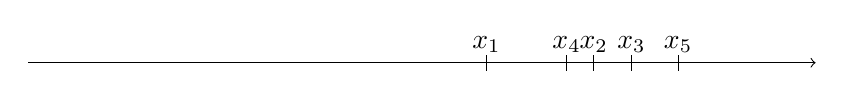
\begin{tikzpicture}[scale=10]
    \draw (0.5820216424559055, -0.01) -- node[above] {$x_1$} (0.5820216424559055, 0.01);
    \draw (0.7181491667223714, -0.01) -- node[above] {$x_2$} (0.7181491667223714, 0.01);
    \draw (0.7661126076135922, -0.01) -- node[above] {$x_3$} (0.7661126076135922, 0.01);
    \draw (0.6837042616132034, -0.01) -- node[above] {$x_4$} (0.6837042616132034, 0.01);
    \draw (0.8252940926247403, -0.01) -- node[above] {$x_5$} (0.8252940926247403, 0.01);
    \draw[->] (0, 0) -- (1, 0);
  \end{tikzpicture}
\end{example}

\begin{itemize}
  \item \textbf{Polynomial}:
    \[
      1 - x - (-x)^{d+1} - \sum_{i = 2}^{d} 2 (-x)^{i} = 0.
    \]
  \item \textbf{Algebraic Solution Vector}:
    \[
      x_i = 2x + (-x)^{i+1} + \sum_{k=2}^{i} (-x)^{k}.
    \]
  \item \textbf{Linear Recurrence}:
    \[
      F(n) = F(n - 1) + (-1)^{d+1} F(n - d) - \sum_{i=2}^{d - 1} (-1)^{i+1} 2 F(n - i).
    \]
  \item \textbf{Rational Solution Vector}:
    \[
      x_1 = \frac{F(n - 1)}{F(n)}, x_i = \frac{2 F(n-1) + (-1)^{i+1} F(n - i) + \sum_{k=2}^i (-1)^k F(n-k)}{F(n)}.
    \]
  \item \textbf{Matrix}:
    \[\left(\begin{array}{cccc|c}
      F(n)   & 0      & \dots  & 0      & F(n - 1) \\
        0    & F(n)   & \dots  & 0      & 2 F(n - 1) - F(n - 2) \\
      \vdots & \vdots & \ddots & \vdots & \vdots   \\
        0    & 0      & \dots  & F(n)   & 2 F(n-1) + (-1)^{d+1} F(n - d) + \sum_{k=2}^d (-1)^k F(n-k) \\
    \end{array}\right)\]
\end{itemize}

\begin{example}
  \begin{align*}
    \left\{ \frac{1}{x_1} \right\}
    & = \left\{ \frac{F(n - 1) + 2 F(n - 2) - 2 F(n - 3) + F(n - 4)}{F(n - 1)} \right\} \\
    & = \frac{2 F(n - 2) - 2 F(n - 3) + F(n - 4)}{F(n - 1)} \\
    \left\{ -\frac{x_2}{x_1} \right\}
    & = \left\{ -\frac{2 F(n - 1) - F(n - 2)}{F(n)} \frac{F(n)}{F(n - 1)} \right\} \\
    & = \frac{F(n - 2)}{F(n - 1)} \\
    \left\{ -\frac{x_3}{x_1} \right\}
    & = \left\{ -\frac{2 F(n - 1) - 2 F(n - 2) + F(n - 3)}{F(n)} \frac{F(n)}{F(n - 1)} \right\} \\
    & = \frac{2 F(n - 2) - F(n - 3)}{F(n - 1)}
  \end{align*}
\end{example}

\section{An Idempotent Solution for Two Dimensions}

Let $\vec x = (\psi, 1 - \psi)$, where $\psi$ is the only real positive root of $x^2 + x - 1$.
For this solution, it does not matter which element we choose to pivot with, it will always
yield the same result.

Pivoting with $x_1$:
\begin{align*}
  \frac{1}{x_1} - 1 & = \frac{1}{\psi} - 1 = \psi, \\
  1 - \frac{x_2}{x_1} & = 1 - \frac{1 - \psi}{\psi} = 1 - \psi.
\end{align*}

Pivoting with $x_2$:
\begin{align*}
  \frac{1}{x_2} - 2 & = \frac{1}{1 - \psi} - 2 = \psi, \\
  1 - \frac{x_1}{x_2} & = 1 - \frac{\psi}{1 - \psi} = 1 - \psi.
\end{align*}

\begin{align*}
  \left(
  \begin{array}{cc|c}
    F(n) & 0    & F(n-1) \\
    0    & F(n) & F(n) - F(n-1) \\
  \end{array}
  \right)
\end{align*}

\section{Bound over Two Iterations}

\begin{proposition}
  In one dimension, the determinant decreases by a factor of at least $1/2$ over
  two iterations.
\end{proposition}

\begin{proof}
  Let $x₁ ∈ ℚ$ be the input to the 1-dimensional algorithm.
  We assume $x₁ > 1/2$ as the other case already proves the assumption.
  Then, $1/x₁ < 2$ and we have
  $$
    x₁ \left\{\frac{1}{x₁}\right\}
    = x₁ \left(\frac{1}{x₁} - 1\right)
    = 1 - x₁ < 1/2.
    $$
  Therefore, over two iterations we decrease by at least $1/2$.
\end{proof}

How can we derive the golden ratio from this?

What can we expect for higher dimensions?
This depends on the strategy of our pivot element $x_\ell$.
There are different strategies we can follow like choosing the minimum in each iteration, for example.

\section{Golden Ratio}

\begin{align*}
  ψ(ψ + 1)^d - 1 = 0,
\end{align*}

Reflecting the polynomial gives us:
\begin{align*}
  φ^{d+1} - (φ + 1)^d = 0.
\end{align*}
Using the binomial theorem:
\begin{align*}
  φ^{d+1} = ∑_{i=0}^d \binom{d}{i} φ^i,
\end{align*}
which leads directly to the Fibonacci numbers for this ratio:
\begin{align*}
  F(n + d + 1) = ∑_{i=0}^d \binom{d}{i} F(n + i).
\end{align*}

We choose $x₁ = ψ$ and $x_i = x₁ (1 + x₁)^{i-1} = ψ (1 + ψ)^{i-1}$.

\begin{align*}
  \text{pivot}(\text{pivot}(x, ℓ₁), ℓ₂) = \left(x_{σ(1)}, \dots, x_{σ(d)}\right).
\end{align*}

From the proof, it follows that $1/(d+1)$ should be the worst-case.
However, using $1/(d+1)$ exactly only requires one iteration until the values are integral.

\begin{align*}
  ψ^{d+1} + ∑_{k=0}^d k ψ^{d-k} = 1.
\end{align*}

Is this the optimal one?

\begin{theorem}
  There is no vector $x ∈ (0, 1)^d$
  such that any pivot operation yields the same decrease
  over every iteration for $d ≥ 2$.
\end{theorem}

\begin{proof}
  Suppose there is such an $x$.
  Then, the distance between neighbors is the same between all elements of $x$.
  This vector is unique.
\end{proof}


\chapter{Hermite's Question}

\begin{problem}[Hermite's Question]
  Is there a representation of the real numbers as a sequence of natural
  numbers such that the sequence is eventually periodic if and only if the real
  number is a cubic irrational?
\end{problem}

More formally: Does there exists a function $f$ which maps any $α ∈ ℝ$ to an
infinite sequence $(a_n)_{n ∈ ℕ}$ of natural numbers such that $a_n$ is
eventually periodic if and only if $α$ is a cubic irrational?
The problem can very easily be generalized to higher degrees of algebraic numbers:
The representation is periodic if and only if $x$ is the root of a polynomial of degree $d + 1$.

\section{Comparison to the Jacobi-Perron Algorithm}

The algorithm in this form, where we always choose the same pivot,
is equivalent to the Jacobi-Perron algorithm, which was first proposed
by Jacobi \cite{Jacobi68} and later analyzed by Perron \cite{Perron07}.
In modern times, the algorithm was picked up again by Bernstein \cite{Bernstein06}.
Each of them has analyzed the algorithm in the context of Hermite's Question.

Charles Hermite initially posed a question to Jacobi, whether there exists a
representation of the real numbers as an infinite sequence of natural numbers
such that the sequence is eventually periodic if and only if the number is a
cubic irrational. The question remains unanswered with the latest attempt
\cite{Murru15} showing that there is an infinite sequence which is eventually
periodic for every cubic irrational.

\section{Finding a Periodic Representation through Brute-Force}

We use the generalized Euclidean algorithm to find a representation for $α ∈ ℝ$.
More specifically, we use the update rule from the algorithm to find the representation.
The update rule takes a vector and not a real number, so we use the vector $x_i = α^i$ for $i ≤ d$.

For our input $x ∈ ℝ^d$, we can build up a $d$-ary tree where $x$ is the root and any
two nodes of this tree $x', x''$ are connected if $\mathrm{pivot}(x, i) = x''$
for some $i$.
The brute-force algorithm performs a breadth-first search over this tree to
find a node which points to a higher node in the tree, i.e. the path forms a loop.
As our pivot sequence we use the path from the root to the this node.

\begin{example}
  The sequences for the prime numbers are:
  \begin{itemize}
    \item $2^{1/3}$: $0\overline{10}$.
    \item $3^{1/3}$: $01\overline{01}$.
    \item $5^{1/3}$: $0\overline{00111000}$.
    \item $7^{1/3}$: $0\overline{010100}$.
    \item $11^{1/3}$: $0\overline{1100}$.
    \item $13^{1/3}$: $00\overline{010000}$.
    \item $17^{1/3}$: $000\overline{11110000}$.
    \item Another choice for $5^{1/3}$ with shorter period: $00110\overline{101010}$.
  \end{itemize}
\end{example}

\begin{remark}
  The first number that has a leading $1$ as the pivot is $12$,
  which has the pivot sequence $1\overline{0111011101}$.
  However, there are other possible choices where it does not have a leading $0$.
\end{remark}

We can likely rule out alternating pivot sequences since this corresponds to
the Jacobi-Perron algorithm and for this algorithm it is conjectured
\cite{Karpenkov2024} that the algorithm is not periodic for $\sqrt[3]{4}$.
However, the brute-force algorithm is periodic for this input (see Table~\ref{table:cube-root-4}).

The choice of the initial input also matters.
We generally choose $x = (α, q(α))$, where $q$ is some polynomial of degree $2$.
But different choices of $q$ produce different sequences.
For example, $(\sqrt[3]{2}, \sqrt[3]{4})$ produces a different sequence of coefficients than $(\sqrt[3]{2}, \sqrt[3]{6})$.
Even though both inputs represent the same number $\sqrt[3]{2}$.
Choosing $q(α) = α^2 - α$ makes the sequence purely periodic for $\sqrt[3]{3}$ and $\sqrt[3]{4}$.

\begin{conjecture}
  The brute-force algorithm is periodic if and only if $α$ is a cubic irrational.
\end{conjecture}

\begin{lemma}
  \label{lem:consecutive-same}
  For every $k ∈ ℕ$, there exists a number $n ∈ ℕ$,
  such that $\sqrt[3]{n}$ and $\sqrt[3]{n + 1}$ have the same first $k$ terms in
  their pivot sequences.
\end{lemma}

\begin{corollary}
  Any strategy which only compares the fractional values does not produce the
  same pivot sequence as the brute-force algorithm.
\end{corollary}

\begin{corollary}
  The minimum strategy does not produce the same pivot sequence as the
  brute-force algorithm.
\end{corollary}

\iffalse
\begin{theorem}
  There exists no algorithm which given $x ∈ ℝ^d$ can determine the same
  strategy as the brute-force search using only $f(d)$ comparison, addition
  and subtraction operations, for some computable function $f \colon ℕ → ℕ$.
\end{theorem}

\begin{proof}
  Idea: A constant-number of additions and subtraction only compare the integer
  parts of each $x_i$ when the values are chosen close enough to an integer.
  Because the trees are the same for the first level, the output for both
  inputs must be the same.

  We choose $x₁ = f(d)$ and $x₂ = \sqrt{f(d) + 1}$ where $n^3 > f(d)$.
  In particular, $x₁$ is an integer and $x₂$ is between $x₁$ and the next integer.
  Suppose the algorithm compares $a₁ x₁$ with $a₂ x₂$ for $|a₁|, |a₂| ≤ f(d)$.
  \[
    a₂ x₂
    = a₂ \sqrt{(f(d))^2 + i + 1}
    ≤ a₂ \left( f(d) + \frac{1}{3 f(d)} \right)
    = a₂ · f(d) + \frac{a₂}{3 f(d)} \right)
  \]
  Furthermore, $a₂ x₂ ≥ a₂ · f(d)$.
  Therefore, the integer part of $a₂ x₂$ is equal to $a₂ x₁$,
  even if $a₂ = f(d)$.
  Hence, any algorithm can only compare the integer parts of $x₁$ and $x₂$.
\end{proof}
\fi

\begin{table}[t]
  \caption{Representation of $ψ = \sqrt[3]{4}$ using the brute-force search.}
  \label{table:cube-root-4}
  \centering
  \begin{tabular}{lllllll}
  \uzlhline
  \uzlemph{$\ell$} & \uzlemph{$x_1$} & \uzlemph{$x_2$} & \uzlemph{$x_1$} & \uzlemph{$x_2$} & \uzlemph{$a_1$} & \uzlemph{$a_2$} \\
	\hline
  $0$ & $\psi$ & $\psi^{2}$ & $1.5874$ & $2.51984$ & $1$ & $2$ \\
  $0$ & $\frac{1}{3} \psi^{2} + \frac{1}{3} \psi + \frac{1}{3}$ & $-\frac{1}{3} \psi^{2} + \frac{2}{3} \psi + \frac{2}{3}$ & $1.70241$ & $0.88499$ & $1$ & $0$ \\
  $1$ & $\frac{1}{4} \psi^{2} + \frac{1}{2} \psi$ & $\frac{1}{2} \psi^{2}$ & $1.42366$ & $1.25992$ & $1$ & $1$ \\
  $0$ & $\frac{1}{4} \psi^{2} + 1$ & $\frac{1}{2} \psi^{2} + \psi + 1$ & $1.62996$ & $3.84732$ & $1$ & $3$ \\
  $0$ & $\psi$ & $\psi^{2} - 2 \psi + 2$ & $1.5874$ & $1.34504$ & $1$ & $1$ \\
  $1$ & $\frac{1}{3} \psi^{2} + \frac{1}{3} \psi + \frac{1}{3}$ & $\psi - 1$ & $1.70241$ & $0.5874$ & $1$ & $0$ \\
  $1$ & $\frac{1}{3} \psi + \frac{2}{3}$ & $\frac{1}{3} \psi^{2} + \frac{1}{3} \psi + \frac{1}{3}$ & $1.1958$ & $1.70241$ & $1$ & $1$ \\
  $0$ & $\frac{1}{12} \psi^{2} - \frac{1}{6} \psi + \frac{1}{3}$ & $\frac{1}{4} \psi^{2} + \frac{1}{2} \psi$ & $0.27875$ & $1.42366$ & $0$ & $1$ \\
  $0$ & $\psi + 2$ & $\psi^{2} - 1$ & $3.5874$ & $1.51984$ & $3$ & $1$ \\
  $0$ & $\frac{1}{3} \psi^{2} + \frac{1}{3} \psi + \frac{1}{3}$ & $-\frac{1}{3} \psi^{2} + \frac{2}{3} \psi + \frac{2}{3}$ & $1.70241$ & $0.88499$ & $1$ & $0$ \\
  \uzlhline
\end{tabular}

\end{table}

\begin{table}[t]
  \caption{Period Length of the first $28$ numbers.}
  \centering
  \begin{tabular}{ll}
  \uzlhline
  \uzlemph{$n^3$} & \uzlemph{Period Length of $n^3$} \\
  \hline
  2 & 2 \\
  3 & 2 \\
  4 & 8 \\
  5 & 8 \\
  6 & 8 \\
  7 & 6 \\
  9 & 2 \\
  10 & 4 \\
  11 & 4 \\
  12 & 10 \\
  13 & 6 \\
  14 & 4 \\
  15 & 6 \\
  16 & 14 \\
  17 & 8 \\
  18 & 6 \\
  19 & 6 \\
  20 & 8 \\
  21 & 8 \\
  22 & 6 \\
  23 & 20 \\
  24 & 8 \\
  25 & 20 \\
  26 & 4 \\
  28 & 2 \\
  \uzlhline
\end{tabular}

\end{table}

\section{Multi-Dimensional Continued Fractions}

\begin{definition}
  Given a sequence of $d$-dimensional vectors $\{rₙ\}_{n ≥ 0}$ and a sequence of
  indices $\{ℓₙ\}_{n ≥ 0}$, the \emph{multi-dimensional fraction} $[r₀; ℓ₁, r₁; …]$ is defined as
  \[
    [r₀] = r₀, \qquad [r₀; ℓ₁, r₁; …; ℓₙ, rₙ] = r₀ + \mathrm{pivot}_{ℓ₁}[r₁; ℓ₂, r₂; …; ℓₙ, rₙ].
  \]
\end{definition}

\begin{remark}~
  \begin{enumerate}
    \item
      The first item has no index.
      The index sequence $ℓₙ$ is always one shorter than the vector sequence $rₙ$.
    \item
      For the generalized Euclidean algorithm, the sequence $r_n$ consists solely of integer vectors.
      However, the MDCF can also be defined over rational or even real vectors.
      To differentiate the two, a sequence $rₙ$ will denote a sequence of real
      vectors and $aₙ$ will denote a sequence of integer vectors.
  \end{enumerate}
\end{remark}

The concepts from one-dimensional continued fractions naturally carry over to its
multi-dimensional counterpart.

\begin{definition}[Complete Quotient, Convergent, Periodicity]~
  \begin{itemize}
    \item The \emph{$k$-th complete quotient} is defined as $[rₖ; r_{k+1}, …]$.
    \item The \emph{$k$-th convergent} of $x$ is defined as the finite fraction $[r₀; ℓ₁, r₁; …; ℓ_k, r_k]$.
    \item The MDCF is \emph{eventually periodic} if there exists $k₀ ≥ 0$ and $ℓ ≥ 1$ such that $rₖ = r_{k+ℓ}$ for every $k ≥ k₀$.
      The MDCF is \emph{purely periodic} if $k₀ = 0$.
  \end{itemize}
\end{definition}

To show that any periodic MDCF contains elements of a field with degree $d + 1$
over the rationals, we proceed similarly to the one-dimensional continued
fraction.
We first show the multi-dimensional analogue of Lemma~\ref{lem:nesting}.

\begin{lemma}[Nesting]
  \label{lem:mdcf-nesting}
  Let $x ∈ ℝ^d$, then
  \[
    [a₀; ℓ₁, a₁; …; ℓₙ, aₙ; ℓ, x]
    = [a₀; ℓ₁, a₁; \cdots; ℓₙ, aₙ + \mathrm{pivot}_{ℓ}(x)]
  \]
\end{lemma}

\begin{proof}
  If $n = 0$, then by definition,
  \[
    [a₀; ℓ, x] = a₀ + \mathrm{pivot}_{ℓ}[x] = a₀ + \mathrm{pivot}_{ℓ}(x) = [a₀ + \mathrm{pivot}_ℓ(x)].
  \]
  Suppose the lemma holds for any $n ≥ 0$, then
  \begin{align*}
    [a₀; ℓ₁, a₁; …; ℓₙ, aₙ; ℓ, x]
    & = a₀ + \mathrm{pivot}_{ℓ₀}[a₁; …; ℓₙ, aₙ; ℓ, x] \\
    & = a₀ + \mathrm{pivot}_{ℓ₀}[a₁; …; ℓₙ, aₙ + \mathrm{pivot}_ℓ(x)] \\
    & = [a₀; ℓ₁, a₁; …; ℓₙ, aₙ + \mathrm{pivot}_ℓ(x)]. \qedhere
  \end{align*}
\end{proof}

In Lemma~\vref{lem:wallis}, we had to define two sequences $pₙ$ and $qₙ$ over
the sequence of the continued fraction $aₙ$.
Each sequence would only return a single scalar.
This time we define two matrix sequences $P^{(n)}, Q^{(n)}$ over the sequences $aₙ$ and $ℓₙ$ as
\begin{align*}
  P_{ℓₙ}^{(n)} & = P_{n-1} a_n + p_{n-1}, & P_i^{(n)} & = P_i^{(n)}, & P^{(-1)}   & = I_d, \\
  Q_{ℓₙ}^{(n)} & = Q_{n-1}^T a_n + q_{n-1}, & Q_i^{(n)} & = Q_i^{(n)}, & Q^{(-1)}_j & = 0,   \\
  p^{(n)}      & = P_{ℓₙ}^{(n-1)},            &           &              & p^{(-1)}_j & = 0,   \\
  p^{(n)}      & = P_{ℓₙ}^{(n-1)},            &           &              & q^{(-1)}   & = 1.
\end{align*}
where $i ≠ ℓ_n$.
What this sequence effectively does is reconstructing the lattice from an
initial solution vector $x ∈ ℝ^d$ and its coefficient vectors $a_n$.

\begin{lemma}[Wallis]
  \label{lem:mdcf-wallis}
  Let $x ∈ ℝ^d$, then
  \[
    [a₀; ℓ₁, a₁; …; ℓ_{n-1}, a_{n-1}; ℓ, x]
    = \frac{P x + p}{Q^T x + q}.
  \]
\end{lemma}

\begin{proof}
  If $n = 0$, then
  \[
    [x] = x = \frac{I_d x + 0}{0^T x + 1}.
  \]
  Suppose the lemma holds for $n ≥ 0$, then there exists a matrix $P$, vectors
  $Q, p$ and scalar $q$ such that
  \begin{align*}
    y & = [a₀; ℓ₁, a₁; …; ℓ_{n-1}, a_{n-1}; ℓ, x]                              \\
      & = [a₀; ℓ₁, a₁; …; ℓ_{n-1}, a_{n-1} + \mathrm{pivot}_ℓ(x)]              \\
      & = \frac{P (a + \mathrm{pivot}_ℓ(x)) + p}{Q^T (aₙ + \mathrm{pivot}_ℓ(x)) + q} \\
      & = \frac{x_ℓ}{x_ℓ} · \frac{P (a + \mathrm{pivot}_ℓ(x)) + p}{Q^T (aₙ + \mathrm{pivot}_ℓ(x)) + q}.
  \end{align*}
  The numerator has the following form:
  \begin{align*}
    x_ℓ (P (a + \mathrm{pivot}(x, ℓ)) + p)
    & = x_ℓ (P a + P_ℓ \frac{1}{x_ℓ} + \sum_{i ≠ ℓ} P_i \frac{x_i}{x_ℓ} + p) \\
    & = \underbrace{(P a + p)}_{P_ℓ'} x_ℓ + \sum_{i ≠ ℓ} \underbrace{P_i}_{P_i'} x_i + \underbrace{P_ℓ}_{p'} \\
    & = P' x + p'.
  \end{align*}
  Analogously, the denominator has the following form:
  \begin{align*}
    x_ℓ (Q^T (a + \mathrm{pivot}(x, ℓ)) + q)
    & = x_ℓ (Q^T a + Q_ℓ \frac{1}{x_ℓ} + \sum_{i ≠ ℓ} Q_i \frac{x_i}{x_ℓ} + q) \\
    & = \underbrace{(Q^T a + q)}_{Q_ℓ'} x_ℓ + \sum_{i ≠ ℓ} \underbrace{Q_i}_{Q_i'} x_i + \underbrace{Q_ℓ}_{q'} \\
    & = Q' x + q'.
  \end{align*}
  Hence,
  \begin{align*}
    y & = \frac{P(a + \mathrm{pivot}(x, ℓ)) + p}{Q(a + \mathrm{pivot}(x, ℓ)) + q} \\
      & = \frac{P' x + p'}{Q'^T x + q'}. \qedhere
  \end{align*}
\end{proof}

\begin{proposition}
  Given $r ∈ ℝ$, let $x = (r¹, r², …, r^d)$.
  If the MDCF representation of $x$ is purely periodic, then $[ℚ(r) : ℚ] ≤ d + 1$.
\end{proposition}

\begin{proof}
  Suppose the algorithm is purely periodic on input $x$ with period $ℓ$.
  Let $y$ be the $ℓ$-th complete quotient of $x$, then $x = y$.
  By Lemma~\ref{lem:mdcf-wallis},
  \[
    rⁱ = \frac{\sum_{j=1}^d P_{ij} rʲ + pᵢ}{\sum_{j=1}^d Qⱼ rʲ + qᵢ}, \text{ for every } i ≤ d.
  \]
  Multiplying both sides with the denominator results in the polynomial equation
  \[
    \sum_{j=1}^d (Q_j r^{i+j} - P_{ij} r^j) + r^i q_i - p_i = 0.
  \]
  For $i = 1$, the maximum degree of this polynomial is $d + 1$.
  Hence, $[ℚ(r) : ℚ] ≤ d + 1$.
\end{proof}

\section{Homogeneous Coordinates}

The pivot operation is quite cumbersome to write.
We'll always need to differentiate the cases $i = ℓ$ and $i ≠ ℓ$.
Homogeneous coordinates allow us to simplify the whole pivot operation as a single matrix.

Instead of an $d$-dimensional vector space, we project each vector into a $(d+1)$-dimensional vector space.
Each vector $x = (x₁, …, x_d) ∈ ℝ^d$ is extended by a new coordinate $x₀ = 1$.
We denote this vector as $\hat x = [1, x₁, …, x_d]$.
Two such vectors $\hat x, \hat y$ are considered equivalent if they are collinear.
Stated differently, each vector $[x₀, x₁, …, x_d]$ represents a line in the direction $(x₀, x₁, …, x_d)$.

% TODO: Explain mapping from and back to the original vector space.
\begin{center}
  \begin{tikzpicture}
    \matrix[
      column sep=2cm,
      nodes={text width=3cm, align=center},
    ] {
      \node (L0) {$\mathbb{R}^d$}; &
      \node (R0) {$\mathbb{RP}^{d+1}$}; \\
      \node (L1) {$(x₁, …, x_d)$}; &
      \node (R1) {$[1, x₁, …, x_d]$}; \\
      \node (L2) {$(x₁/x₀, …, x_d/x₀)$}; &
      \node (R2) {$[x₀, x₁, …, x_d]$}; \\
    };

    \draw[->] (L1) -- node[above] {} (R1);
    \draw[<-] (L2) -- node[above] {} (R2);
  \end{tikzpicture}
\end{center}

For example, consider the vector $[1, x₁, x₂]$ with $0 ≤ x₁, x₂ < 1$.
A pivot operation with $ℓ = 1$ would result in the vector $[1, 1/x₁, x₂/x₁]$.
This vector is equivalent to $[x₁, 1, x₂]$.
Therefore, we can reformulate this operation as a coordinate swap of $x_ℓ$ with
the new coordinate $x₀$:
\[
  \begin{bmatrix}
    0 & 1 & 0 \\
    1 & 0 & 0 \\
    0 & 0 & 1 \\
  \end{bmatrix}
  ·
  \begin{bmatrix} 1 \\ x₁ \\ x₂ \\ \end{bmatrix}
  =
  \begin{bmatrix} x₁ \\ 1 \\ x₂ \\ \end{bmatrix}.
\]
Similarly, subtracting the integer part of each value in $[1, x₁, x₂]$ is
equivalent to a series of skew operations:
\[
  \begin{bmatrix}
    1 & 0 & 0 \\
    -\floor{x₁} & 1 & 0 \\
    0 & 0 & 1 \\
  \end{bmatrix}
  ·
  \begin{bmatrix}
    1 & 0 & 0 \\
    0 & 1 & 0 \\
    -\floor{x₂} & 0 & 1 \\
  \end{bmatrix}
  ·
  \begin{bmatrix} 1 \\ x₁ \\ x₂ \\ \end{bmatrix}
  =
  \begin{bmatrix} 1 \\ x₁ - \floor{x₁} \\ x₂ - \floor{x₂} \\ \end{bmatrix}.
\]
Importantly, each of those matrices with
determinant $1$.
Therefore, the whole operation can be reversed by inverting the matrix.
This is the equivalent of the inverse pivot operation in homogeneous
coordinates.

We can also reformulate the MDCF as a series of matrix multiplications.
In the following $T(a)$ denotes the translation by a vector $a ∈ ℝ^d$
and the matrix $S(ℓ)$ denotes the swap of $x_\ell$ with $x_0$.
The MDCF can then be written as
\[
  [a₀] = \hat a₀, \qquad
  [a₀; ℓ₁, a₁; …; ℓₙ, aₙ] = T(a₀) · S(ℓ_1) · [a₁; ℓ_2, a_2; …; ℓ_n, a_n].
\]

This allows us to drastically simplify Lemma~\ref{lem:mdcf-wallis}.
Now, we only have a single matrix sequence $P_n$, defined as follows:
\begin{align*}
  P_n = P_{n-1} A_n, \qquad P_0 = I_{d+1}.
\end{align*}

\begin{lemma}
  \label{lem:mdcf-wallis'}
  Let $x ∈ ℝ^d$, then
  \[
    [a₀; ℓ₁, a₁; …; ℓ_{n-1}, a_{n-1}; ℓ, x] = P_{n-1} \hat x
  \]
\end{lemma}

\begin{proof}
  For $n = 0$, this is clearly true.
  Suppose the lemma is true for $n ≥ 0$, then
  \begin{align*}
    [a₀; ℓ₁, a₁; …; ℓ_n, a_n; ℓ, x]
    & = [a₀; ℓ₁, a₁; …; ℓ_n, a_n + \mathrm{pivot}_ℓ(x)] \\
    & = P_{n-1}
    \begin{pmatrix}
      a_n + \mathrm{pivot}_ℓ(x) \\ 1
    \end{pmatrix} \\
    & = P_{n-1} A_n \hat{x} \\
    & = P_n \hat{x} \qedhere
  \end{align*}
\end{proof}

\begin{theorem}
  Let $A ∈ ℤ^{d×d}, B ∈ ℤ^d$ and $C ∈ ℤ$.
  If $x^\top A x + B x + C = 0$ for some vector $x ∈ ℝ^d$,
  then the MDCF of $x$ is eventually periodic.
\end{theorem}

\begin{proof}

\end{proof}

\begin{corollary}
  If $r$ is the root of a polynomial of degree $2d$,
  then the MDCF of $x = (r^1, …, r^d)$ is eventually periodic.
\end{corollary}

\chapter{Experimental Analysis of the Periodicity}

\section{Finding a Periodic Representation through Brute Force}

% TODO: Maybe replace this with the pseudocode instead?
\begin{minipage}{0.48\textwidth}
\begin{Python}[basicstyle=\small\ttfamily, frame={}]
def brute_force_search(xs, max_depth):
    d = len(xs)
    for L in sequences(d, max_depth):
        ys = tuple(xs)
        index = {ys: 0}
        for i, l in enumerate(L):
            ys = pivot(ys, l)
            if ys in index:
                j = index[ys]
                start = L[:j]
                period = L[j:i+1]
                return start, period
            else:
                index[ys] = i + 1
\end{Python}
\end{minipage}
\vrule width 1pt
\hfill
\begin{minipage}{0.48\textwidth}
\begin{Python}[basicstyle=\small\ttfamily, frame={}]
def sequences(base, max_digits):
    seq = []
    while True:
        carry = 1
        for i in range(len(seq) - 1, -1, -1):
            seq[i] += carry
            if seq[i] == base:
                seq[i] = 0
                carry = 1
            else:
                carry = 0
                break
        if carry:
            if len(seq) < max_digits:
                seq.insert(0, 1)
            else:
                break
        yield seq[1:]
\end{Python}
\end{minipage}

\section{Results for Cubic Irrationals}

\begin{example}
  The sequences for the prime numbers are:
  \begin{itemize}
    \item $2^{1/3}$: $0\overline{10}$.
    \item $3^{1/3}$: $01\overline{01}$.
    \item $5^{1/3}$: $0\overline{00111000}$.
    \item $7^{1/3}$: $0\overline{010100}$.
    \item $11^{1/3}$: $0\overline{1100}$.
    \item $13^{1/3}$: $00\overline{010000}$.
    \item $17^{1/3}$: $000\overline{11110000}$.
    \item Another choice for $5^{1/3}$ with shorter period: $00110\overline{101010}$.
  \end{itemize}
\end{example}

\begin{remark}
  The first number that has a leading $1$ as the pivot is $12$,
  which has the pivot sequence $1\overline{0111011101}$.
  However, there are other possible choices where it does not have a leading $0$.
\end{remark}

\begin{table}[t]
  \caption{Representation of $ψ = \sqrt[3]{4}$ using the brute-force search.}
  \label{table:cube-root-4}
  \centering
  \begin{tabular}{lllllll}
  \uzlhline
  \uzlemph{$\ell$} & \uzlemph{$x_1$} & \uzlemph{$x_2$} & \uzlemph{$x_1$} & \uzlemph{$x_2$} & \uzlemph{$a_1$} & \uzlemph{$a_2$} \\
	\hline
  $0$ & $\psi$ & $\psi^{2}$ & $1.5874$ & $2.51984$ & $1$ & $2$ \\
  $0$ & $\frac{1}{3} \psi^{2} + \frac{1}{3} \psi + \frac{1}{3}$ & $-\frac{1}{3} \psi^{2} + \frac{2}{3} \psi + \frac{2}{3}$ & $1.70241$ & $0.88499$ & $1$ & $0$ \\
  $1$ & $\frac{1}{4} \psi^{2} + \frac{1}{2} \psi$ & $\frac{1}{2} \psi^{2}$ & $1.42366$ & $1.25992$ & $1$ & $1$ \\
  $0$ & $\frac{1}{4} \psi^{2} + 1$ & $\frac{1}{2} \psi^{2} + \psi + 1$ & $1.62996$ & $3.84732$ & $1$ & $3$ \\
  $0$ & $\psi$ & $\psi^{2} - 2 \psi + 2$ & $1.5874$ & $1.34504$ & $1$ & $1$ \\
  $1$ & $\frac{1}{3} \psi^{2} + \frac{1}{3} \psi + \frac{1}{3}$ & $\psi - 1$ & $1.70241$ & $0.5874$ & $1$ & $0$ \\
  $1$ & $\frac{1}{3} \psi + \frac{2}{3}$ & $\frac{1}{3} \psi^{2} + \frac{1}{3} \psi + \frac{1}{3}$ & $1.1958$ & $1.70241$ & $1$ & $1$ \\
  $0$ & $\frac{1}{12} \psi^{2} - \frac{1}{6} \psi + \frac{1}{3}$ & $\frac{1}{4} \psi^{2} + \frac{1}{2} \psi$ & $0.27875$ & $1.42366$ & $0$ & $1$ \\
  $0$ & $\psi + 2$ & $\psi^{2} - 1$ & $3.5874$ & $1.51984$ & $3$ & $1$ \\
  $0$ & $\frac{1}{3} \psi^{2} + \frac{1}{3} \psi + \frac{1}{3}$ & $-\frac{1}{3} \psi^{2} + \frac{2}{3} \psi + \frac{2}{3}$ & $1.70241$ & $0.88499$ & $1$ & $0$ \\
  \uzlhline
\end{tabular}

\end{table}

\begin{table}[t]
  \caption{Period Length of the first $28$ numbers.}
  \centering
  \begin{tabular}{ll}
  \uzlhline
  \uzlemph{$n^3$} & \uzlemph{Period Length of $n^3$} \\
  \hline
  2 & 2 \\
  3 & 2 \\
  4 & 8 \\
  5 & 8 \\
  6 & 8 \\
  7 & 6 \\
  9 & 2 \\
  10 & 4 \\
  11 & 4 \\
  12 & 10 \\
  13 & 6 \\
  14 & 4 \\
  15 & 6 \\
  16 & 14 \\
  17 & 8 \\
  18 & 6 \\
  19 & 6 \\
  20 & 8 \\
  21 & 8 \\
  22 & 6 \\
  23 & 20 \\
  24 & 8 \\
  25 & 20 \\
  26 & 4 \\
  28 & 2 \\
  \uzlhline
\end{tabular}

\end{table}

\section{Results for Quartic and Higher-Degree Irrationals}

\section{Evaluation of More Efficient Search Strategies}

We can likely rule out alternating pivot sequences since this corresponds to
the Jacobi-Perron algorithm and for this algorithm it is conjectured
\cite{Karpenkov21} that the algorithm is not periodic for $\sqrt[3]{4}$.
However, the brute-force algorithm is periodic for this input (see Table~\ref{table:cube-root-4}).

The choice of the initial input also matters.
We generally choose $x = (α, q(α))$, where $q$ is some polynomial of degree $2$.
But different choices of $q$ produce different sequences.
For example, $(\sqrt[3]{2}, \sqrt[3]{4})$ produces a different sequence of coefficients than $(\sqrt[3]{2}, \sqrt[3]{6})$.
Even though both inputs represent the same number $\sqrt[3]{2}$.
Choosing $q(α) = α^2 - α$ makes the sequence purely periodic for $\sqrt[3]{3}$ and $\sqrt[3]{4}$.

\chapter{Conclusion and Outlook}
\label{ch:conclusion}

The main objective of this thesis
was to investigate Hermite's question
on a new representation of real numbers,
which is periodic if and only if the number is algebraic.
The basis for this representation has been a generalization of Euclidean
algorithm by \citeauthor{Klein24}.
Specifically, I have used a small subroutine from the algorithm,
which was used to update the old solution vector instead of solving a linear
system in each iteration.
This subroutine was then used as the basis of the multidimensional continued fractions.
Although these were not enough to fully solve Hermite's question,
we have seen that many concepts from the Euclidean algorithm naturally carry
over to its generalization.

Beginning with the Fibonacci numbers,
we saw that different strategies lead to different definitions of Fibonacci numbers.
The first example of such numbers was for the minimum strategy,
which chooses the smallest fractional value.
For this strategy, the $d$-bonacci numbers represent the worst case,
just like the Fibonacci numbers represent the worst case for the classical
Euclidean algorithm.
The second strategy improves upon this strategy by minimizing the ratio between two values over two iterations.
For this strategy, its golden ratio and the corresponding Fibonacci numbers
already came up when bounding the decrease of the determinant over just two iterations.
Although the golden ratio is not periodic under the strategy itself,
we have seen that the maximum strategy leads to periodicity.
These two roots were the first examples of periodic inputs for the generalized Euclidean algorithm.

These examples led to the development of multidimensional continued fractions
as presented in Chapter~\ref{ch:mdcf}.
They are essentially the generalized Euclidean algorithm, but in reverse.
Since the algorithm allows us to choose a pivot index at each iteration,
there does not exist a unique multidimensional continued fraction for every vector.
However, this choice provides more flexibility.
Instead of focusing on a single algorithm, the multidimensional continued
fractions unify many Jacobi-Perron-type algorithms under one framework.
Additionally, they share many properties with continued fractions.
For example, the linear recurrence for continued fractions proven in Lemma~\ref{lem:cf-wallis}
has an equivalent sequence proven in Lemma~\ref{lem:mdcf-wallis} for
multidimensional continued fractions.

The convergence of multidimensional continued fractions was proven in Section~\ref{sec:mcf-convergence}.
The proof is considerably more complex than for continued fractions.
However, it still shows that the multidimensional continued fractions are
converging under any algorithm, which chooses all possible pivot indices and
chooses these indices not too far apart.
This covers algorithms like the classical Jacobi-Perron algorithm,
but also other algorithms, which choose the pivot indices based on a fixed list.
Most importantly, it establishes the first part of Hermite's question.
It shows that many algorithms lead to a representation of the real numbers
using the multidimensional continued fractions.

While the first part of Hermite's question has been solved,
the second part is only partially solved.
Whereas the first part only asks of a representation of the real numbers,
the second part states that the repersentation should be periodic if and only
if the number is a cubic irrational (or algebraic number, in general).
The first direction has been proven in Section~\ref{sec:mcf-periodic}.
The proof is based on eigenvectors and shows that if the MCF of an irrational vector $x$ is
purely periodic, then $x$ is one of the eigenvectors in the convergent matrix.
% TODO: We have to define the convergent matrix

Theorem~\ref{thm:unimodular-algebraic} suggests that we can always find a
unimodular matrix with $x$ as one of its eigenvectors,
thereby indicating that we should be able to find a periodic MCF.
However, I was not able to show this in the scope of this thesis.
Nevertheless, the analysis in Chapter~\ref{ch:implementation}
strongly supports the conjecture.
In particular, the algorithm by \citeauthor{Tamura09} has shown promise for
finding periodic representation of cubic and quartic irrationals.
The authors have already proven that their algorithm is periodic for certain
classes of cubic polynomials.
Future research into this algorithm could possibly lead to a periodic sequence
for all cubic and quartic irrationals.

In the case of continued fractions,
we were able to show that they are periodic only if the number is a quadratic irrational.
The proof uses Klein polygons, which are preserved under a specific unimodular transformation
and we can find such a transformation for every quadratic irrational.
We can find a similar transformation for all algebraic numbers, but for the
multidimensional continued fractions we are missing the connection between them
and Klein polytopes.
Section~\ref{sec:mdcf-geometry} already provides the necessary foundation for this.
Furthermore, there already exists a generalization of Lagrange's theorem by
\citeauthor{German08}~\cite{German08}.

% TODO: Add note about how approximation doesn't work well with the multi-dimensional continued fractions


\begin{bibtex-entries}
@article{Murru15,
  title     = {On the periodic writing of cubic irrationals and a generalization of R{\'e}dei functions},
  author    = {Murru, Nadir},
  journal   = {International Journal of Number Theory},
  volume    = {11},
  number    = {03},
  pages     = {779--799},
  year      = {2015},
  publisher = {World Scientific}
}

@book{Bernstein06,
  title     = {The Jacobi-Perron algorithm: Its theory and application},
  author    = {Bernstein, Leon},
  volume    = {207},
  year      = {2006},
  publisher = {Springer}
}

@article{Perron07,
  title     = {Grundlagen f{\"u}r eine Theorie des Jacobischen Kettenbruchalgorithmus},
  author    = {Perron, Oskar},
  journal   = {Mathematische Annalen},
  volume    = {64},
  number    = {1},
  pages     = {1--76},
  year      = {1907},
  publisher = {Springer}
}

@article{Jacobi68,
  title   = {Allgemeine Theorie der kettenbruch{\"a}hnlichen Algorithmen, in welchen jede Zahl aus drei vorhergehenden gebildet wird.},
  author  = {Jacobi, CGJ},
  journal = {Journal f{\"u}r die reine und angewandte Mathematik},
  volume  = {69},
  pages   = {29--64},
  year    = {1868}
}

@article{Karpenkov2024,
  title     = {On a periodic Jacobi--Perron type algorithm},
  author    = {Karpenkov, Oleg},
  journal   = {Monatshefte f{\"u}r Mathematik},
  volume    = {205},
  number    = {3},
  pages     = {531--601},
  year      = {2024},
  publisher = {Springer}
}
\end{bibtex-entries}

\end{document}
